\documentclass[a4paper,12pt,oneside,openany,titlepage]{book}
\usepackage{amssymb}
\usepackage{ucs}
\usepackage[utf8x]{inputenc}
%\usepackage[polish]{babel}
\usepackage{polski}
\usepackage[OT4]{fontenc}
\usepackage{amsmath}
\usepackage{amsfonts}
\usepackage[T1]{fontenc}
\usepackage{graphicx}
\graphicspath{ {images/} }
\usepackage{tabu}
\usepackage{pgfplots}
 
\pagestyle{headings}
 
\begin{document}

\chapter{Wstęp}

Celem niniejszej pracy inżynierskiej było zaimplementowanie i wdrożenie systemu
wczesnego wykrywania ataków sieciowych typu DDoS w środowisku sieci sterowanych
programowo SDN. Najważniejszymi założeniami projektowymi były: poprawna
implementacja algorytmu do wykrywania ataku DDoS oraz możliwość skalowania
systemu celem zwiększenia jego wydajności.

Architektura systemu zaprojektowanego na potrzeby niniejszej pracy zakłada
umieszczenie stworzonego oprogramowania na połudiowym interfejsie sieci SDN jako
osobny jej komponent oraz, że cały ruch pomiędzy przełącznikami SDN, a
kontrolerem SDN będzie przechodził przez wspomiany komponent. Takie podejście
umożliwia umieszczenie oprogramowania na osobnej maszynie, co z kolei daje
możliwość skalowania systemu poprzez budowanie klastra złożonego z wielu
instancji komponentu, a także ułatwia konfigurację sieci (nie ma potrzeby
ingerencji w inne urządzenia sieciowe). Ponadto umiejscowienie oprogramowania
pomiędzy przełącznikami, a kontrolerem umożliwa analizowanie wiadomości
protokołu \textit{OpenFlow} wymienianych pomiędzy tymi urządzeniami. Analiza
tychże wiadomości jest wykorzystywana przez zaimplementowany algorytm wykrywania
ataku DDoS.

Algorytm służacy do wykrywania ataku DDoS zaimplmentowany we wspomianym systemie
bazuje na entropii pakietów w sieci. Spadek entropii oznacza spadek losowości
pakietow. W przypadku ataku DDoS duża ilość pakietów w sieci skierowana
jest do pojedycznego węzła końcowego, powodując spadek losowości pakietów, tym
samym powodując spadek entropii. Wspomniany algorytm bazuje na opisanej
zależności. W celu obliczenia entropii analizowane są wiadomości
\textit{PACKET\_IN} protokołu \textit{OpenFlow} wysyłane przez przełączniki SDN
do kontrolera SDN.

Wydajność systemu została zapewniona dzięki zastosowaniu technologi
wspierających programowanie równoległe oraz budowę systemów rozproszonych.
Wykorzystane zostały funkcyjne języki programowania Erlang oraz Elixir. Oba te
języki działają na Maszynie Wirtualnej Erlanga (\textit{BEAM}), która dostarcza
natywne wsparcie na wspomianych technologi. Dzięki temu stworzone oprogramowanie
może obsługiwać wiele przełączników w tym samym czasie oraz działać w klastrze.

W celu sprawdzenia czy założenia projektowe zostały spełnione wykonano serie
testów. Sprawdzono czy proces wykrywania ataku DDoS działa prawidłowo zarówno z
wykrzystaniem jednego węzła oprogramowania, jak i rozpraszając ten proces na
kilka węzłów. Ponadto przetestowano możliwość horyzontalnego skalowania całego
systemu.

\chapter{Wybrane aspekty bezpieczeństwa w sieciach SDN }
\chaptermark{Wybrane aspekty bezp. w sieciach SDN}

Ostatnimi czasy, sieci sterowane programowo (SDN) zdobywają popularność zarówno
w środowiskach akademickich, jak również wśród komercyjnych przedsiębiorstw.
Zcentralizowany model zarządzania siecią, jaki wprowadzono w architekturze SDN
fundamentalnie zmienił spojrzenie na sposób zarządzania w sieciach rozproszonych
\cite{ddosNYarticle}. Sieci SDN dostarczają nowych możliwości w zakresie
monitorowania sieci, a co za tym idzie, również w zakresie wykrywania ataków
sieciowych, m.in. ataków typu DDoS (z ang. \textit{distributed
  denial-of-service}). Niniejszy rozdział przybliża ideę sieci SDN oraz wybrane
sposoby wykrywania ataków DDoS. 

\section{Sieci sterowane programowo SDN}
Sieci sterowane programowo (z ang. \textit{Software Defined Networking})
wprowadzają rozdział warstwy danych od warstwy zarządzającej oraz wprowadzają
centralny punkt zarządzania siecią, który jest w pełni programowalny \cite{onf}.
Innymi słowy, możliwe jest zaprogramowanie konfiguracji sieci. Warstwa danych,
jest odpowiedzialna tylko i wyłącznie za przełączanie danych, wedle reguł
otrzymanych od warstwy zarządzającej. Do warstwy danych należą przełączniki SDN.
Warstwa zarządzająca natomiast, jest odpowiedzialna za podejmowanie wszelkiego
rodzaju decyzji związanych z działaniem sieci, np. określa jak powinny być
przełączane/rutowane pakiety w sieci. Urządzeniem warstwy zarządzającej jest
kontroler SDN. Kontroler komunikuje się z przełącznikami z wykorzystaniem tzw.
południowego interfejsu \cite{sdninterfaces}.

Komunikacja pomiędzy przełącznikami, a kontrolerem w sieci SDN odbywa się z
wykorzystaniem protokołu \textit{OpenFlow}. Jest on obecnie szeroko stosowany w
dzisiejszych sieciach SDN \cite{ddoskoreaarticle}. Przełącznik SDN przełącza
pakiety zgodnie z tablicą przepływów (z ang. \textit{flow table}). Przepływ
charakteryzuje pewną grupę podobnych pakietów, np. mających taki sam adres
docelowy \textit{IP}. Każda reguła w tablicy przepływów określa jaką akcję
przełącznik powinien podjąć w związku z danymi należącymi do danego
przepływu, np. przełączyć je na port X. Tablica przepływów jest zarządzana przez
kontroler sieci SDN.

Przełącznik oraz kontroler komunikują się ze sobą z wykorzystaniem
predefiniowanych wiadomości protokołu \textit{OpenFlow}. W przypadku, gdy
przełącznik nie znajduje reguły w tablicy przepływów pasującej do ramki/pakietu,
którą otrzymał, wysyła wiadomość \textit{PACKET\_IN} protokołu
\textit{OpenFlow}, do kontrolera. Kontroler podejmuje decyzję co zrobić z danym 
pakietem/ramką i przekazuje tę informację do przełącznika za pomocą wiadomości
\textit{PACKET\_OUT}. Następnie instaluje nowy przepływ w tablicy przepływów
przełącznika, aby mógł on przełączać podobne pakiety/ramki bez konieczności
udziału kontrolera. W tym celu kontroler wysyła do przełącznika wiadomość
\textit{FLOW\_ADD}. Protokół \textit{OpenFlow} definiuje o wiele więcej
wiadomości, jednakże nie ma konieczności ich omawiania na potrzeby niniejszej
pracy inżynierskiej.

\section{Bezpieczeństwo sieci SDN w kontekście ataku DDoS}

Sieci SDN są nadal stosunkowo nową koncepcją, która nie jest jeszcze w
powszechnym użyciu, ale wraz ze wzrostem zainteresowania tą technologią oraz
powszechności użycia, sieci SDN staną się w niedalekiej przyszłości celem ataków
\cite{sdnsecurityblog}. W tym podrozdziale zostanie omówiona kwestia
bezpieczeństwa sieci SDN w kontekście ataku DDoS.

Atak DDoS jest rodzajem ataku sieciowego, w którym atakujący wykorzystuje wiele
węzłów sieciowych np. zainfekowanych komputerów do wygenerowania ruchu
sieciowego adresowanego do konkretnego węzła końcowego. W efekcie atakowany
węzeł wykazuje większe latencje lub w ogóle przestaje odpowiadać na żądania,
ponieważ jest całkowicie zaabsorbowany obsługą fałszywego ruchu.

W przypadku sieci SDN, atak DDoS powoduje dodatkowe problemy w sieci. W
niektórych pracach naukowych atak ten jest nazywany \textit{SDN-DDoS}
\cite{ddosbronksarticle}: sieć SDN jest zalana ruchem, który nie należy do
żadnego znanego przełącznikom w sieci przepływu (jest wręcz losowy). W takiej
sytuacji, każdy przełącznik, który obsługuje fałszywy ruch wysyła wiadomości
\textit{PACKET\_IN} do kontrolera w celu obsługi nieznanych (fałszywych)
pakietów. Taka sytuacja powoduje szereg implikacji: prawdziwy ruch sieciowy jest
obsługiwany wolniej lub w ogóle, ponieważ kontroler jest zajęty przetwarzaniem
fałszywego ruchu \cite{indiaarticle}. Ponadto, do kontrolera jest wysyłana duża
liczba wiadomości \textit{PACKET\_IN}, co może doprowadzić do jego przeciążenia.
W przypadku awarii kontrolera cała sieć SDN przestaje być użyteczna
\cite{ddoskoreaarticle}. Z wyż. wym. powodów wczesne wykrycie ataku DDoS w
sieciach SDN ma kluczowe znaczenie dla poprawnego działania całej sieci. 

\section{Metody wykrywania ataków DDoS w sieciach SDN}

Ataki DDoS w kontekście sieci SDN budzą duże zainteresowanie w środowisku
akademickim. Pojawiło się dość sporo artykułów naukowych prezentujących rozmaite
metody wykrywania tego typu ataków. Opisane zostały zarówno bardzo podstawowe
metody bazujące na entropii, jak również te bardziej zaawansowane. Na potrzeby
niniejszej pracy przywołano i pokrótce opisano wybrane metody wykrywania
ataków DDoS. 

Jedna z metod przedstawiona w \cite{ddosNYarticle} opisuje sposób wykrywania
ataku bazujący na monitorowaniu natężenia ruchu dla poszczególnych przepływów, a
także ich asymetrii, tzn. monitorowania natężenia ruchu w obie strony: zarówno
ruchu do potencjalnej ofiary, jak i od niej. Dzięki takiemu podejściu możliwe
jest odróżnienie naturalnych przepływów o wysokim natężeniu np. transfer danych
pomiędzy centrami danych od przepływów odpowiedzialnych za atak DDoS.
Wykorzystanie wspomnianej metody opisano na dwa sposoby, jako \textit{Metodę
  Sekwencyjną} oraz \textit{Metodę Równoległą}. 

Kolejna metoda zaprezentowana w \cite{ddoskoreaarticle} bazuje na czynnikach
związanych z czasem. Badacze we wspomnianym artykule zaprojektowali metodę
wykrywania ataku DDoS wykorzystującą ilość czasu jaki upłynął zanim ruch
osiągnął pewien stopień natężenia, wzorce czasowe ataków DDoS oraz docelowe
adresy pakietów w sieci. Wspomniana ilość czasu związana z natężeniem ruchu jest
wykorzystywana do wykrycia ataku DDoS, natomiast wzorce czasowe mają zapobiegać
atakom w przyszłości. Metody wykorzystujące informację o długości trwania ataku
są rzadko stosowane \cite{ddoskoreaarticle}. 

Metoda wykrywania ataków DDoS bazująca na entropii została opisana w
\cite{mainddosarticle}. Entropia jest obliczana na podstawie docelowych adresów
\textit{IP} poszczególnych pakietów w sieci. Jest ona obliczana dla zadanej
długości okna, które składa się z ustalonej liczby pakietów. Gdy obliczona
entropia spadnie poniżej zadanego poziomu dla kilku następujących po sobie okien
uznaje się, że w sieci nastąpił atak. Algorytm ten został zaimplementowany w
projekcie wykonanym na potrzeby niniejszej pracy inżynierskiej. Został on
szczegółowo opisany w rozdziale \ref{algorithm} strona \pageref{algorithm}.

System wykrywania ataków DDoS opisany w \cite{bloomarticle} jest w stanie wykryć
typ ataków skierowanych na poszczególne łącze w sieci. Tego typu atak ma na celu
wysycenie konkretnego łącza. Proponowane rozwiązanie bazuje na analizie tablic
przepływów oraz pakietów w sieci SDN. Opisywany system składa się z dwóch
elementów: \textit{Collector}'a oraz \textit{Detector}'a. \textit{Collector} ma
za zadanie skanować tablice przepływów w sieci w celu znalezienia podejrzanych
przepływów (odpowiedzialnych za wysycenia łącza). Podejrzane przepływy są
zapisywane w specjalnej strukturze danych, na potrzeby której wykorzystano Filtr
Blooma \footnote{https://en.wikipedia.org/wiki/Bloom\_filter}.
Odpowiedzialnością \textit{Detecor}'a jest skanowanie sieci w celu pozyskania
pakietów do analizy. Następnie komponent sprawdza, czy dany pakiet należy do
któregoś z podejrzanych przepływów i wysyła odpowiednie powiadomienie do
kontrolera SDN.

\chapter{Wydajność systemów ochrony sieciowej przed atakami DDoS}

\chapter{Projekt i jego implementacja}

\chapter{Weryfikacja rozwiązania}

W celu weryfikacji poprawności działania zaiplementowanego systemu zostały
wykonane serie testów. System został przetestowany pod kątem sprawdzenia
podstawowych założeń projektowych tj. poprawności wykrywania anomali, związanych
z natężeniem ruchu, w obsługiwanej sieci oraz możliwości skalowania
aplikacji \textit{sdn\_epc} w celu zwiększenia wydjaności systemu.
Przeprowadzenie testów wymagało przygotowania odpowiednich scenariuszy testowych,
zestawienia dedykowanych topolgi sieciowych oraz stworzenia rozwiązań
pozwalających na zebranie własciwych danych z testowanego systemu. Analiza
tychże wyników pozwoliła na stwierdzenie, czy i w jakim stopniu założenia
projektowe zostały spełnione. Niniejszy rozdział szczegółowo opisuje
poszczególne przypadki testowe oraz prezentuje analizę uzyskanych wyników.

\section{Test działania implementacji algorytmu}

% w jaki sposób sprawdzamy czy algorytm działa? Liczymy entropie, trzeba to
% ująć
 
Aby stwierdzić, czy zaimplementowany algorytm (\pageref{equ:entropy}) w aplikacji
\textit{sdn\_epc} spełnia swoją rolę tzn. pozwala wykryć atak DDoS w sieci SDN
zostały przeanalizowane wartości entropii obliczone za pomocą tegoż właśnie
algorytmu w dwóch różnych przypadkach testowych, z których każdy wykorzystywał
nieco inną konfigurację testową topologi sieciowej, jak również samej aplikacji
\textit{sdn\_epc}. Przetestowane zostały przypadki, gdy: 
\begin{enumerate}
  \item Ruch wygenerowany w sieci testowej był obsługiwany tylko przez jeden
    węzeł aplikacji \textit{sdn\_epc}.
  \item Ruch wygenerowanych w sieci testowej był obsługiwany przez wiele węzłów
    aplikacji \textit{sdn\_epc} działających w klastrze.
\end{enumerate}
Wykorzystanie takich właśnie przypadków testowych umożliwiło sprawdzenie
poprawności implementacji algorytmu zarówno w przypadku działania systemu jako
pojedynczy węzeł aplikacji \textit{sdn\_epc}, jak również w przypadku, gdy
system działał w klastrze. Drugi przypadek jest znacznie bardziej złożony,
ponieważ rozproszenie procesu obliczania algorytmu na wiele węzłów wprowadza
dodatkowe komplikacje, związane z synchronizacją stanu pomiędzy węzłami w
klastrze.

\subsection{Przypadek testowy z wykorzystaniem jednego węzła aplikacji
  \textit{sdn\_epc}} \label{entropy_one_node}

Schemat topologii sieciowej, wykorzystanej w przypadku, gdy tylko jeden węzeł
aplikacji jest zaangażowany w przetwarzenie ruchu został przedstawiony na
Rys. \ref{fig:entropia_scheme}.

\begin{figure}[h]
\centering
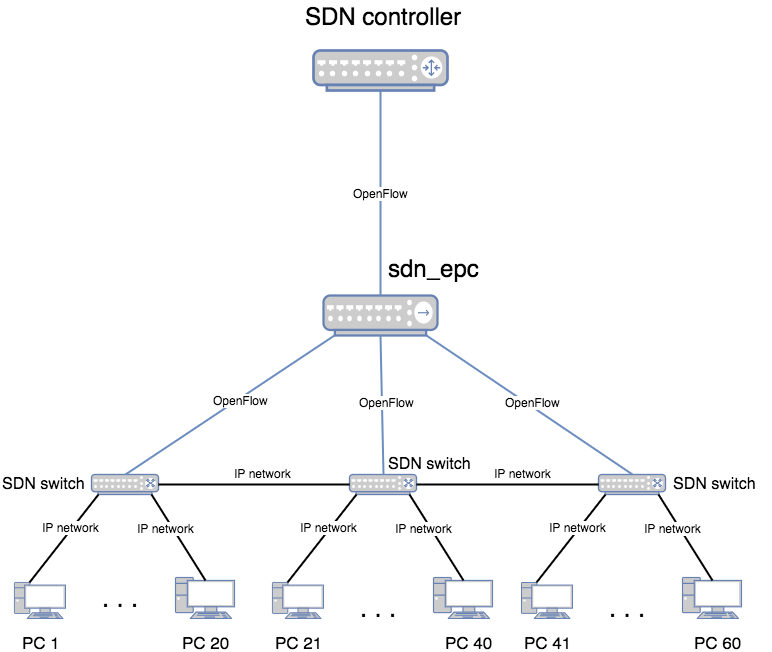
\includegraphics[width=\textwidth]{entropia_scheme}
\caption{Schemat topologii sieciowej z wykorzystaniem jednego węzła aplikacji
  \textit{sdn\_epc}}
\label{fig:entropia_scheme}
\end{figure}

W topologii przedstawionej na Rys. \ref{fig:entropia_scheme} wszystkie
przełączniki obsługujące ruch pomiędzy węzłami końcowymi (\textit{PC N})
komunikują się z kontrolerem (\textit{SDN controller}) poprzez jeden węzeł
aplikacji \textit{sdn\_epc}. Wykorzystując taką konfigurację sieci, tylko jeden
węzeł \textit{sdn\_epc} przetwarza wiadomości \mbox{\textit{PACKET\_IN}}
protokołu \textit{OpenFlow}, wymieniane pomiędzy poszczególnymi przełącznikami,
a kontrolerem, w celu obliczenia entropii pakietów przesyłanych w sieci.

Jeśli algorytm został poprawnie zaimplementowany to wartość entropii,
obliczonej za jego pomocą, powinna maleć wzraz ze spadkiem losowości pakietów
przesyłanych w sieci testowej. Innymi słowy, im więcej pakietów w sieci jest
adresowanych do pojedynczego węzła końcowego, tym mniejsza będzie wartość
obliczonej entropii.

W celu sprawdzenia czy wspomiana zależność została spełniona, koniecznym było
zaprojektowanie odpowiedniego scenariusza testowego. Scenariusz ten opierał się
na środowisku testowym przedstawionym na Rys. \ref{fig:entropia_tech}.

\begin{figure}[h]
\centering
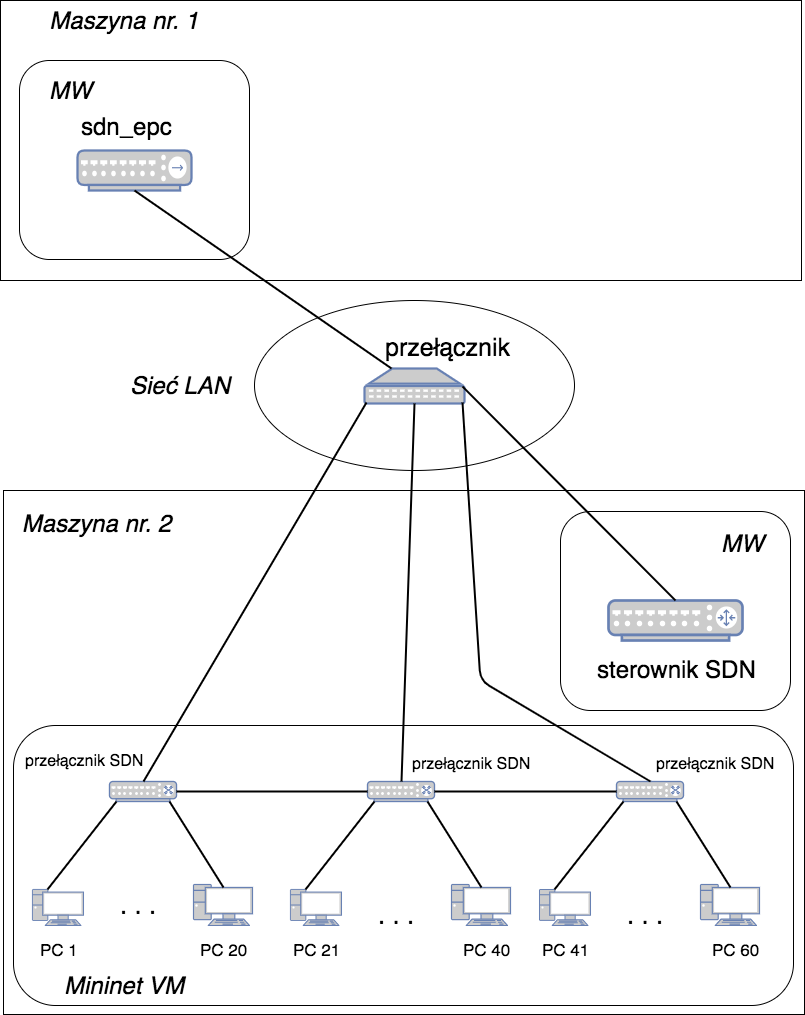
\includegraphics[height=11cm]{entropia_tech}
\caption{Środowisko testowe z wykorzystaniem jednego węzła aplikacji
  \textit{sdn\_epc}}
\label{fig:entropia_tech}
\end{figure}

Jak przedstawiono na Rys. \ref{fig:entropia_tech} toplogia sieciowa została
zestawiona z użyciem dwóch maszyn fizycznych, na których zostały zwirtualizowane
niezbędne komponenty testowe. Każdy z komponentów, za wyjątkiem przełącznika
sieci \textit{LAN} (\textit{switch}), został uruchomiony na dedykowanej maszynie
wirtualnej. Jako środowisko do wirtualizacji zostało wykorzystane oprogramowanie
\textit{VirtualBox \footnote{https://www.virtualbox.org}}. Maszyny wirtualne
komunikowały się ze sobą z wykorzystaniem sieci \textit{LAN}.

Przełączniki sieci SDN (\textit{SDN switch}'es) oraz węzły końcowe (\textit{PC
  N}) były emulowane na dedykowanej maszynie wirtualnej za pomocą oprogramowania
\textit{Mininet \footnote{http://mininet.org}}. Wykorzystane w teście
przełączniki to domyślne przełączniki używane przez oprogramowanie
\textit{Mininet}, które działają na bazie oprogramowania
\textit{Open vSwitch \footnote{http://openvswitch.org}}.
\textit{SDN controller}, pełniący funkcję kontrolera w testowej topologii,
korzystał z oprogramowania zbudowanego z wykrzystaniem framework'a
\textit{Ryu \footnote{https://osrg.github.io/ryu}}. Maszyny wirtualne dedykowane
dla \textit{sdn\_epc} i \textit{SDN controller} działały pod kontrolą systemu
operacyjnego \textit{Ubuntu \footnote{https://www.ubuntu.com}}.

Scenariusz testowy zakładał przeprowadzenie kilku prób, podczas których w sieci
były generowane ataki DDoS o różnej sile. Podczas każdej próby została zmierzona
średnia wartość entropii obliczonej za pomocą zaimplementowanego algorytmu.
Wykonane zostały cztery próby z atakami o sile odpowiednio: 0\%, 30\%, 60\% oraz
90\%. Siła każdego ataku została obliczona na podstawie wzoru
\ref{equ:ddos_power}

\begin{equation}
R = \frac{P_{a}}{P_{n}} \cdot 100\%
\label{equ:ddos_power}
\end{equation}
gdzie R oznacza siłę ataku, $P_{a}$ pakiety atakujące, natomiast $P_{n}$ pakiety
tła.

Pakiety tła rozumiane są jako pakiety
\textit{IP \footnote{https://tools.ietf.org/html/rfc791\#section-3.1}} wysyłane
do losowo wybranych węzłów końcowych w stałych odstępach czasowych. Pakiety
atakujące oznaczają pakiety \textit{IP}, które zawierają losowe adresy docelowe
oraz są wysyłane do konkretnego węzła końcowego w 4-krotnie krótszych odstępach
czasowych niż pakiety tła. 

Podczas każdej próby wybrane węzły końcowe generowały pakiety tła oraz
pakiety atakujące (jeden węzeł generował jeden typ pakietów). Do generowania
pakietów została wykorzystana biblioteka języka \textit{Python} o nazwie
\textit{ Scapy \footnote{http://www.secdev.org/projects/scapy}}. Szczegółowe
dane opisujące każdą z prób zostały przedstawione w Tab. \ref{tab:entropy}.
\newpage

\begin{table}[h!]
\centering
\begin{tabular}{ |c|c|c|c|c| } 
 \hline
 R & $P_{n}$ & $P_{a}$ & interwał $P_{n}$ & interwał $P_{a}$ \\
 \hline
 0\% & 3000 & 0 & 20ms & 5ms \\ 
 \hline
 30\% & 3000 & 900 & 20ms & 5ms \\ 
 \hline
 60\% & 3000 & 1800 & 20ms & 5ms \\ 
 \hline
 90\% & 3000 & 2700 & 20ms & 5ms \\ 
 \hline
\end{tabular}
\caption{Parametry prób testowych z wykorzystaniem jednego węzła aplikacji
  \textit{sdn\_epc}} 
\label{tab:entropy}
\end{table}

Warto zaznaczyć, że średnio 3,4\% wszystkich pakietów z danej próby nie dotarło
do aplikacji \textit{sdn\_epc}. Wydaje się, że nie powinno wpływać to znacząco
na uzyskane wyniki, jednak, ze względu na fakt, że przeprowadzenie tego typu
testów wymaga znacznych zasobów obliczeniowych, do których dostęp nie jest
ogólnodostępny, wpływ wspomianego zjawiska nie został naukowo zbadany.

Na wykresie \ref{plot:entropy} przedstawiono średnią wartość entropii,
obliczonej przez aplikację \textit{sdn\_epc} przy użyciu zaimplementowanego w
niej algorytmu, dla poszczególnych prób testowych.

\begin{figure}[h]
\centering
\begin{tikzpicture}
\begin{axis}[
    xlabel={Siła ataku [\%]},
    ylabel={Średnia wartośc entropi},
    xmin=0, xmax=100,
    ymin=0.7, ymax=1.2,
    xtick={0,20,40,60,80,100},
    ytick={0.7,0.8,0.9,1,1.1,1.2},
    legend pos=outer north east,
    ymajorgrids=true,
    grid style=dashed,
]
 
\addplot[
    color=blue,
    mark=square,
    ]
    coordinates {
    (0,1.164)(30,1.025)(60,0.891)(90,0.748)
    };
    \legend{jeden węzeł \textit{sdn\_epc}}
 
\end{axis}
\end{tikzpicture}
\caption{Średnia wartość entropii w zależności od siły ataku DDoS}
\label{plot:entropy}
\end{figure}

Zależność entropii od siły ataku, przedstawiona na wykresie \ref{plot:entropy},
jest taka, jak przewidywano. Wzraz ze wzorstem siły ataku wartość entropii
maleje, ponieważ im większa siła ataku, tym większy procent wszystkich pakietów
w sieci trafia do jednego, atakowanego, węzła końcowego. W związku z tym,
losowość poszczególnych pakietów spada, tym samym powodując spadek entropii
pakietów w sieci.

Bazując na przestawionych wynikach i ich analizie, można stwiedzić, że alogorytm
służacy do wykrywania ataku DDoS, został poprawnie zaimplementowany w aplikacji
\textit{sdn\_epc} i umożliwa wykrycie tego typu anomali. 

\subsection{Przypadek testowy z wykorzystaniem kilku węzłów aplikacji
  \textit{sdn\_epc} działających w klastrze}

Schemat topologii sieciowej wykorzystanej w przypadku, gdy kilka węzłów
aplikacji \textit{sdn\_epc} działających w klastrze obsługuje ruch w sieci
został zaprezentowany na Rys. \ref{fig:entropia_multi_scheme}.

\begin{figure}[h]
\centering
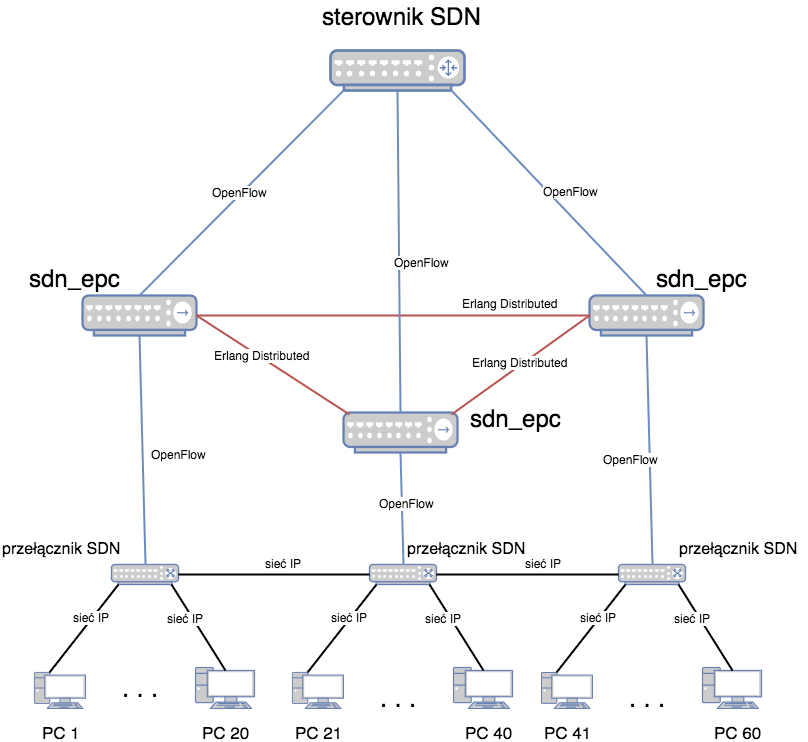
\includegraphics[width=\textwidth]{entropia_multi_scheme}
\caption{Schemat topologii sieciowej z wykorzystaniem trzech węzłów aplikacji
  \textit{sdn\_epc} działających w klastrze}
\label{fig:entropia_multi_scheme}
\end{figure}

Topologia przedstawiona na Rys. \ref{fig:entropia_multi_scheme} jest bardzo
podobna do przedstawionej na Rys. \ref{fig:entropia_scheme} na stronie
\pageref{fig:entropia_scheme}. W tym przypadku, każdy przełącznik w sieci
komunikuje się z kontrolerem poprzez dedykowany węzeł aplikacji
\textit{sdn\_epc}, a więc w klastrze działa dokładnie tyle węzłów
\textit{sdn\_epc} ile jest przełączników w sieci. Każdy węzeł aplikacji obsłguje
tylko tylko jeden przełącznik. Najważniejszą różnica, względem przypadku, gdy
tylko jeden węzeł aplikacji obsłguje wszystkie przełączniki w sieci, jest
rozproszenie procesu obliczania entropii na wiele węzłów \textit{sdn\_epc}.

W związku z tym, że rozposzenie procesu obliczania entropii na wiele węzłów,
wprowadziło szereg komplikacji, które należło uwzględnić, aby poprawnie ją
obliczyć, zostały przeprowadzene dokładnie takie same próby testowe, jak opisano
w sekcji \ref{entropy_one_node} ale z wykorzystaniem innej topologii testowej.
Przeporwadzenie bliźniaczych prób pozwoliło porównać wyniki, tj. wartości
entropii, w przypadku obliczania jej z użyciem jednego (patrz wykres
\ref{plot:entropy} strona \pageref{plot:entropy}) oraz kilku węzłów
\textit{sdn\_epc}. Takie porównanie pozwoliło ustalić, czy zaimplementowany
algorytm działa poprawnie również w przypadku rozproszenia procesu obliczania
entropii.
\newpage

Środowisko przygotowane na potrzeby przeprowadzenia prób testowych, z
wykorzystaniem kilku węzłow \textit{sdn\_epc} przedstawiono na Rys.
\ref{fig:entropy_multi_tech}.

\begin{figure}[h]
\centering
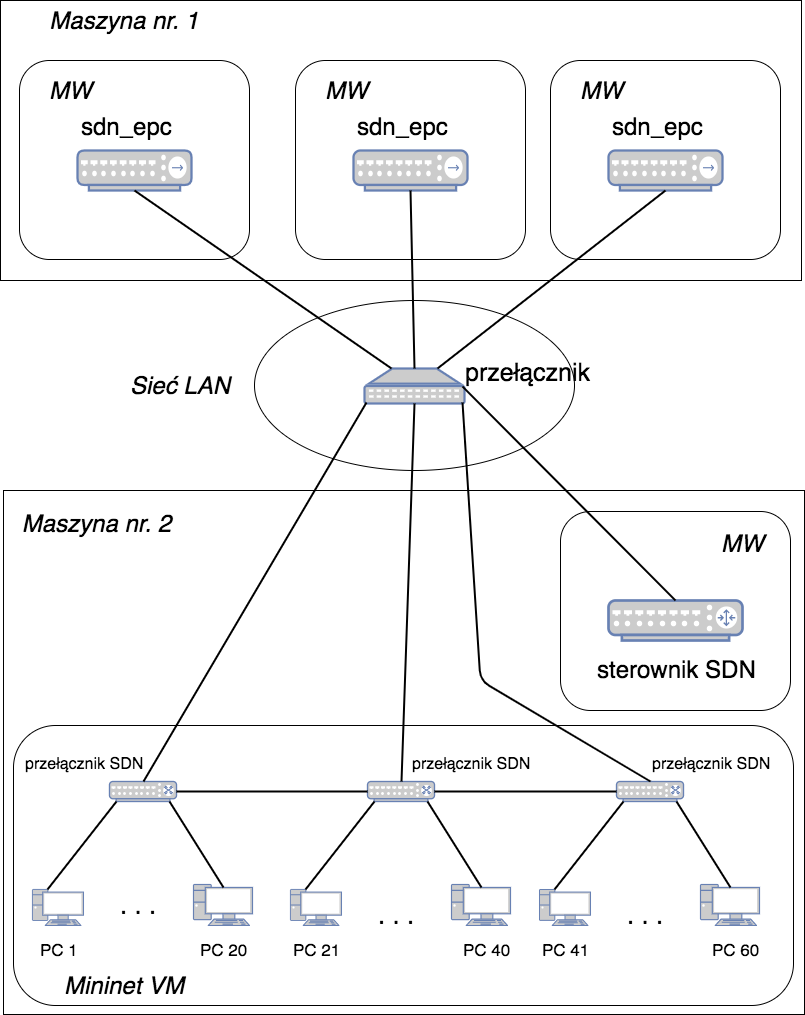
\includegraphics[height=11cm]{entropy_multi_tech}
\caption{Środowisko testowe z wykorzystaniem trzech węzłów aplikacji
  \textit{sdn\_epc} działających w klastrze}
\label{fig:entropy_multi_tech}
\end{figure}

Testowa topologia sieciowa przedstawiona na Rys. \ref{fig:entropy_multi_tech}
została zbudowana z takich samych komponentów i wykorzystując dokładnie takie
same rozwiązania i technologie jak przedstawiono na Rys. \ref{fig:entropia_tech}
strona \pageref{fig:entropia_tech} oraz opisano w sekcji \ref{entropy_one_node}.

W celu zmierzenia średniej wartości entropii z wykorzystaniem wielu węzłów
aplikacji \textit{sdn\_epc} przeprowadzono takie same próby testowe jak opisano
w Tab. \ref{tab:entropy} strona \pageref{tab:entropy}. Uzyskane wyniki zostały
przedstawione na wykresie \ref{plot:entropy_multi_node} wraz z wynikami
pozyskanymi przy próbach z wykorzystaniem jednego węzła \textit{sdn\_epc}, aby
umożliwić porównanie wyników otrzymanych z użyciem dwóch topolgii sieciowych.

\begin{figure}[h]
\centering
\begin{tikzpicture}
\begin{axis}[
    xlabel={Siła ataku [\%]},
    ylabel={Średnia wartośc entropi},
    xmin=0, xmax=100,
    ymin=0.7, ymax=1.2,
    xtick={0,20,40,60,80,100},
    ytick={0.7,0.8,0.9,1,1.1,1.2},
    legend pos=outer north east,
    ymajorgrids=true,
    grid style=dashed,
]

\addplot[
    color=blue,
    mark=square,
    ]
    coordinates {
    (0,1.164)(30,1.025)(60,0.891)(90,0.748)
    };
    \addlegendentry{jeden węzeł \textit{sdn\_epc}}

\addplot[
    color=red,
    mark=*,
    ]
    coordinates {
    (0,1.171)(30,1.027)(60,0.903)(90,0.746)
    };
    \addlegendentry{trzy węzły \textit{sdn\_epc}}

\end{axis}
\end{tikzpicture}
\caption{Średnia wartość entropii dla różnych konfiguracji testowych w
  zależności od siły ataku DDoS}
\label{plot:entropy_multi_node}
\end{figure}


\chapter{Podsumowanie}

\chapter{Wykaz tabel}

\end{document}